\documentclass[a4paper,11pt]{exam}
	\usepackage{graphicx}
	\usepackage[utf8]{inputenc}
	\usepackage[T1]{fontenc}
	\usepackage{listings}
	\usepackage{color}
	\usepackage{amsmath}
	\usepackage{enumerate}
	\usepackage{caption}
	\usepackage{verbatim}
	\usepackage{subcaption}
	\usepackage{tikz}
	\usepackage{graphics}
	\usepackage{txfonts}
	\usepackage{listings}
	\definecolor{dkgreen}{rgb}{0,0.5,0}
	\definecolor{gray}{rgb}{0.5,0.5,0.5}
	\definecolor{mauve}{rgb}{0.58,0,0.82}

	\lstset{frame=tb,
	  language=Python,
	  aboveskip=3mm,
	  belowskip=3mm,
	  showstringspaces=false,
	  columns=flexible,
	  basicstyle={\small\ttfamily},
	  numbers=none,
	  numberstyle=\tiny\color{gray},
	  keywordstyle=\color{blue},
	  commentstyle=\color{dkgreen},
	  stringstyle=\color{mauve},
	  breaklines=true,
	  breakatwhitespace=true
	  tabsize=3
	  }
\begin{document}
\begingroup 
	  \bf \Large Eletromagnetismo\\
	  \indent \normalsize André Del Bianco Giuffrida
	\endgroup
	\\ \quad
	\\
	\large{
	\emph{Lista 3 \\ Ex 7}
        \\
        \\
	\indent Uma carga pontual $q$ está localizada a uma altura $x_0$ entre dois planos condutores paralelos e aterrados, situados em $x=0$ e $x=d$.
	\\
	\\
	\indent (a) Determine a posição das infinitas cargas-imagem necessárias para expressar o potencial elétrico entre as placas.
	\\
	\indent (b) Expresse o potencial e a força elétrica que atua sobre $q$ como séries infinitas em função da posição $x_0$ da carga.
	\normalsize
	
	\begin{center}
		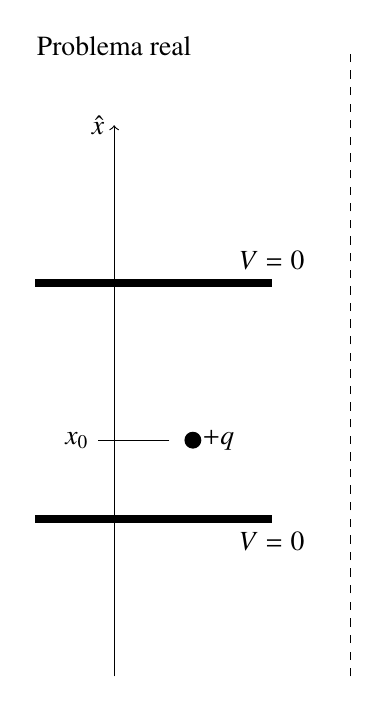
\begin{tikzpicture}
			\draw (0,6) node {Problema real};
			
			\draw[line width=1mm] (-1,0) -- (2,0) node[below] {$V=0$};
			\draw[line width=1mm] (-1,3) -- (2,3) node[above] {$V=0$};
			\draw[arrows=->] (0,-2) -- (0,5) node[left] {$\hat{x}$};
			\draw[fill=black] (1,1) circle (0.1) node[right] {$+q$};
			\draw[dashed] (3,-2) -- (3,6);
			\draw (0.7,1) -- (-0.2,1) node[left] {$x_0$} ;
		\end{tikzpicture}
		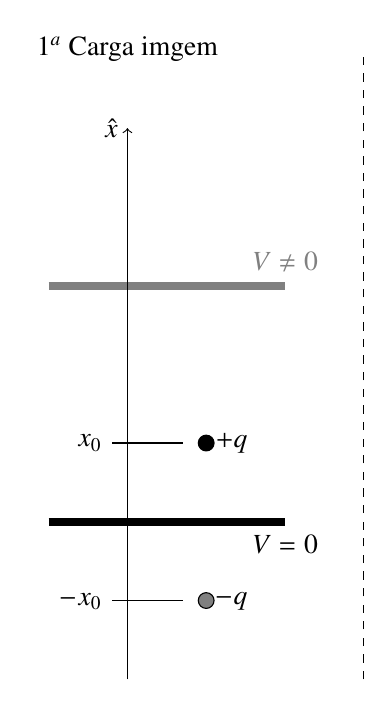
\begin{tikzpicture}
			\draw (0,6) node {$1^a$ Carga imgem};
		  	\draw[line width=1mm] (-1,0) -- (2,0) node[below] {$V=0$};
			\draw[gray, line width=1mm] (-1,3) -- (2,3) node[above] {$V\ne0$};
			\draw[arrows=->] (0,-2) -- (0,5) node[left] {$\hat{x}$};
		  	\draw[fill=black] (1,1) circle (0.1) node[right] {$+q$};
		  	\draw[fill=gray] (1,-1) circle (0.1) node[right] {$-q$};
		  	\draw (0.7,1) -- (-0.2,1) node[left] {$x_0$} ;
		  	\draw (0.7,-1) -- (-0.2,-1) node[left] {$-x_0$} ;
		  	\draw[dashed] (3,-2) -- (3,6);
		\end{tikzpicture}
		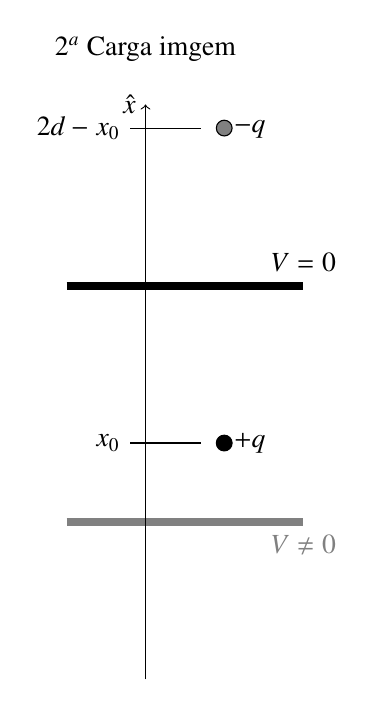
\begin{tikzpicture}
			\draw (0,6) node {$2^a$ Carga imgem};
		  	\draw[gray, line width=1mm] (-1,0) -- (2,0) node[below] {$V \ne 0$};;
			\draw[line width=1mm] (-1,3) -- (2,3) node[above] {$V=0$};
			\draw[arrows=->] (0,-2) -- (0,5.3) node[left] {$\hat{x}$};
		  	\draw[fill=black] (1,1) circle (0.1) node[right] {$+q$};
		  	\draw[fill=gray] (1,5) circle (0.1) node[right] {$-q$};
		  	\draw (0.7,1) -- (-0.2,1) node[left] {$x_0$} ;
		  	\draw (0.7,5) -- (-0.2,5) node[left] {$2d - x_0$} ;
		\end{tikzpicture}
	\end{center}
	
	Afim de manter o potencial $V=0$ nas duas placas podemos continuar neste raciocinio.
	
	\begin{center}
		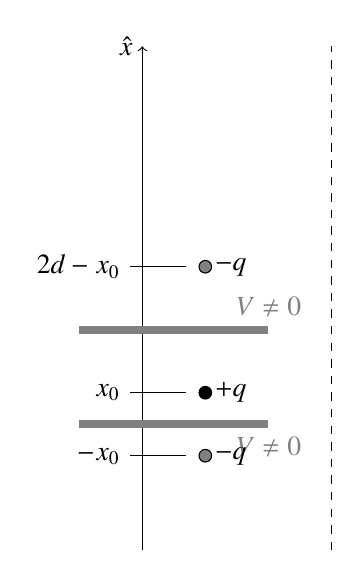
\begin{tikzpicture}[scale=0.8]
			%Config
		  	\draw[dashed] (3,-2) -- (3,6);
			\draw[arrows=->] (0,-2) -- (0,6) node[left] {$\hat{x}$};
			\draw[fill=black] (1,0.5) circle (0.1) node[right] {$+q$}; %Carga inicial
			\draw (0.7,0.5) -- (-0.2,0.5) node[left] {$x_0$} ;
			
			%Planos
		  	\draw[gray, line width=1mm] (-1,0) -- (2,0) node[below] {$V \ne 0$};
		  	\draw[gray, line width=1mm] (-1,1.5) -- (2,1.5) node[above] {$V \ne 0$};
		  	
		  	%Cargas imagem e seus labels
		  	\draw[fill=gray] (1,-0.5) circle (0.1) node[right] {$-q$};
		  	\draw (0.7,-0.5) -- (-0.2,-0.5) node[left] {$-x_0$} ;
		  	\draw (0.7,2.5) -- (-0.2,2.5) node[left] {$2d - x_0$} ;
		  	\draw[fill=gray] (1,2.5) circle (0.1) node[right] {$-q$};
		\end{tikzpicture}
		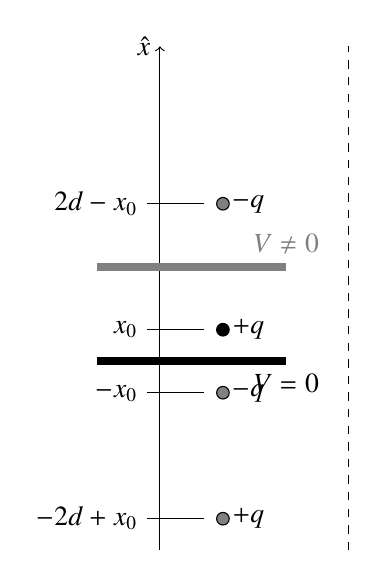
\begin{tikzpicture}[scale=0.8]
			%Config
		  	\draw[dashed] (3,-3) -- (3,5);
			\draw[arrows=->] (0,-3) -- (0,5) node[left] {$\hat{x}$};
			\draw[fill=black] (1,0.5) circle (0.1) node[right] {$+q$}; %Carga inicial
			\draw (0.7,0.5) -- (-0.2,0.5) node[left] {$x_0$} ;
			
			%Planos
			%x=1.5
		  	\draw[gray, line width=1mm] (-1,1.5) -- (2,1.5) node[above] {$V \ne 0$};
		  	%x=0
		  	\draw[ line width=1mm] (-1,0) -- (2,0) node[below] {$V = 0$};
		  	
		  	%Cargas imagem e seus labels
		  	
		  	\draw[fill=gray] (1,-0.5) circle (0.1) node[right] {$-q$};
		  	\draw (0.7,-0.5) -- (-0.2,-0.5) node[left] {$-x_0$} ;
		  	
		  	\draw[fill=gray] (1,2.5) circle (0.1) node[right] {$-q$};
		  	\draw (0.7,2.5) -- (-0.2,2.5) node[left] {$2d - x_0$} ;
		  	
		  	\draw[fill=gray] (1,-2.5) circle (0.1) node[right] {$+q$};
		  	\draw (0.7,-2.5) -- (-0.2,-2.5) node[left] {$-2d + x_0$} ;
		  	
		\end{tikzpicture}
		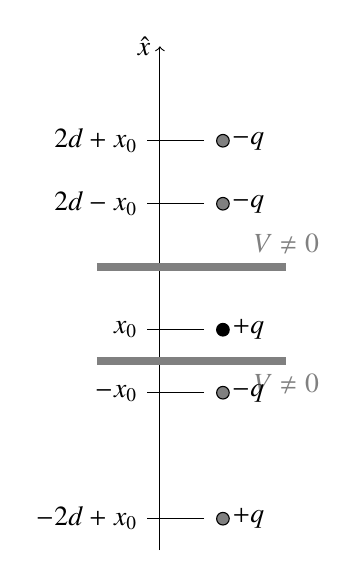
\begin{tikzpicture}[scale=0.8]
			%Config
			\draw[arrows=->] (0,-3) -- (0,5) node[left] {$\hat{x}$};
			\draw[fill=black] (1,0.5) circle (0.1) node[right] {$+q$}; %Carga inicial
			\draw (0.7,0.5) -- (-0.2,0.5) node[left] {$x_0$} ;
			
			%Planos
			%x=1.5
		  	\draw[gray, line width=1mm] (-1,1.5) -- (2,1.5) node[above] {$V \ne 0$};
		  	%x=0
		  	\draw[gray, line width=1mm] (-1,0) -- (2,0) node[below] {$V \ne 0$};
		  	
		  	%Cargas imagem e seus labels
		  	
		  	\draw[fill=gray] (1,-0.5) circle (0.1) node[right] {$-q$};
		  	\draw (0.7,-0.5) -- (-0.2,-0.5) node[left] {$-x_0$} ;
		  	
		  	\draw[fill=gray] (1,2.5) circle (0.1) node[right] {$-q$};
		  	\draw (0.7,2.5) -- (-0.2,2.5) node[left] {$2d - x_0$} ;
		  	
		  	\draw[fill=gray] (1,-2.5) circle (0.1) node[right] {$+q$};
		  	\draw (0.7,-2.5) -- (-0.2,-2.5) node[left] {$-2d + x_0$} ;
		  	
		  	\draw[fill=gray] (1,3.5) circle (0.1) node[right] {$-q$};
		  	\draw (0.7,3.5) -- (-0.2,3.5) node[left] {$2d + x_0$} ;
		\end{tikzpicture}
				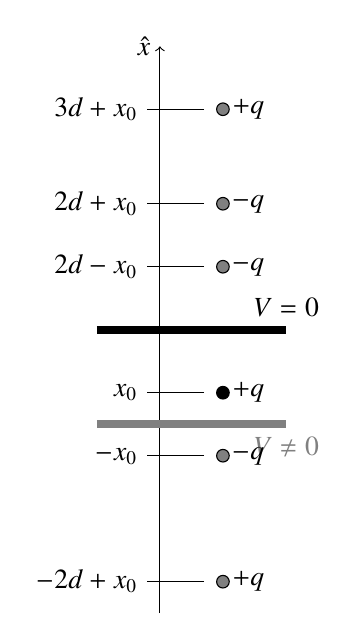
\begin{tikzpicture}[scale=0.8]
			%Config
			\draw[arrows=->] (0,-3) -- (0,6) node[left] {$\hat{x}$};
			\draw[fill=black] (1,0.5) circle (0.1) node[right] {$+q$}; %Carga inicial
			\draw (0.7,0.5) -- (-0.2,0.5) node[left] {$x_0$} ;
			
			%Planos
			%x=1.5
		  	\draw[line width=1mm] (-1,1.5) -- (2,1.5) node[above] {$V = 0$};
		  	%x=0
		  	\draw[gray, line width=1mm] (-1,0) -- (2,0) node[below] {$V \ne 0$};
		  	
		  	%Cargas imagem e seus labels
		  	
		  	\draw[fill=gray] (1,-0.5) circle (0.1) node[right] {$-q$};
		  	\draw (0.7,-0.5) -- (-0.2,-0.5) node[left] {$-x_0$} ;
		  	
		  	\draw[fill=gray] (1,2.5) circle (0.1) node[right] {$-q$};
		  	\draw (0.7,2.5) -- (-0.2,2.5) node[left] {$2d - x_0$} ;
		  	
		  	\draw[fill=gray] (1,-2.5) circle (0.1) node[right] {$+q$};
		  	\draw (0.7,-2.5) -- (-0.2,-2.5) node[left] {$-2d + x_0$} ;
		  	
		  	\draw[fill=gray] (1,3.5) circle (0.1) node[right] {$-q$};
		  	\draw (0.7,3.5) -- (-0.2,3.5) node[left] {$2d + x_0$} ;
		  	
		  	\draw[fill=gray] (1,5) circle (0.1) node[right] {$+q$};
		  	\draw (0.7,5) -- (-0.2,5) node[left] {$3d + x_0$} ;
		\end{tikzpicture}
		
	\end{center}

	Podemos admitir uma equação generica para o potencial no plano em $x=0$ e em $x=d$:
	
	\[V_n(0) = \frac{1}{4 \pi \epsilon_0} (-1)^n \]


\end{document}
